\documentclass[aps,onecolumn,preprintnumbers,amsmath,amssymb,nofootinbib,superscriptaddress,notitlepage]{revtex4-1}

\usepackage{epsfig}
\usepackage[utf8]{inputenc}
\usepackage[dvipsnames]{xcolor}
\usepackage[normalem]{ulem}
%\usepackage{slashed}
\usepackage{caption}
\usepackage{amssymb}
\usepackage{mathtools}
\usepackage{bbold}
\usepackage{amssymb,latexsym}
\usepackage{amsmath,amsbsy,bbm}

\newcommand{\reales}{{\rm R}\hspace{-1ex}\rule{0.1mm}{1.5ex}\hspace{1ex}}
\def\tstrut{\vrule height2.5ex depth0pt width0pt} % used in tables
\def\jtstrut{\vrule height5ex depth0pt width0pt} % used in tables


\newcommand{\eftnopi}{\mbox{EFT$(\not \! \pi)$}}

\definecolor{green}{HTML}{2E8B57}
\interfootnotelinepenalty=10000 %% Completely prevent breaking of footnote

\begin{document}


%\title{Universally emergent L=1 resonances}
\title{Four-body L=1 systems from contact EFT}

\author{Lorenzo Contessi}\email{lorenzo@contessi.net}
\address{IRFU, CEA, Universit\'e Paris-Saclay, 91191 Gif-sur-Yvette, France}

\author{Jaume Carbonel}
\address{Universit\'e Paris-Saclay, CNRS/IN2P3, IJCLab, 91405 Orsay, France}

\author{Johannes Kirscher}
\address{Theoretical Physics Division, School of Physics and Astronomy,\\
  The University of Manchester, Manchester, M13 9PL, UK}
  
\author{Rimantas Lazauskas}
\address{IPHC, IN2P3-CNRS/Universit\'e de Strasbourg BP 28, F-67037 Strasbourg Cedex 2, France}

\author{Martin Sch{\"a}fer}
\address{Nuclear Physics Institute of the Czech Academy of Sciences, 25069 \v{R}e\v{z}, Czech Republic}

\date{\today}


\begin{abstract} 
Scattering resonances are ubiquitous in physics, and for the understanding of the behaviour of few-body quantum systems as important as bound states.
Compared with the latter, their theoretical handling and their role in
the interpretation of data is complicated through their unstable nature
which is reflected in their wave functions not being elements of a
square-integrable space.
The smallest nuclear system comprised solely of resonances
is 4-hydrogen with $L=1$ states about $3.5$~MeV above the triton-neutron
threshold.

In this article, we analyze the minimal contact theory which predicts
such $P$-wave, four-body resonances. Furthermore, we establish numerically
the emergence of this specific resonance pole for a wider class of systems
whose two-body scale is significantly larger ($\to\infty$) compared with the
interaction range.
Specifically, we employ a contact effective field theory renormalized
with nuclear observables -- in which case the interaction is identical
to the leading order of the pionless effective field theory --
and to unitary systems without a finite two-body scale (universal
contact effective field theory). We find a negative-parity four-body
resonance pole which is stable with respect to the short-distance structure
of the regularized two- and three-body momentum-independent contact
potentials with three independent numerical algorithms: a finite-volume
Gaussian-stochastic-variational technique, the solution of the AGS on a
discrete coordinate-space grid, and a one-channel, two-body,
resonating-group reduction of the problem.
Thereby we demonstrate that a zero-range potential
provides a non-trivial pole structure for the four-body amplitude.
\end{abstract}



\maketitle

\section{Introduction}

Resonance phenomena occur ubiquitously in quantum and classical physics.
Relative to stable bound states, their handling in many-particle hadronic, nuclear,
and atomic physics is complicated. 
A resonance results from a nonperturbative interplay of particle-particle interactions,
fine-tuned potential shapes, and channel couplings that lead to multiple
excitations and thresholds.
Relative long life times and energies very close to production thresholds lead to
clean, measurable signals, while in practise, a rapid decay and an energy far from
threshold makes their identification with cross section data involved. 
Theoretically, the structure of a Hamiltonian usually does not expose the existence of
resonances without explicitly solving dynamical equations. In the latter course,
numerical methods to extract complex energies are, in general, expensive and
less accurate compared with those for bound states.
%

%
In order to identify general features of an interaction which allow for the
prediction of resonances, we focus on the smallest nuclear system, known to
be characterized by a resonance, namely, the 4-hydrogen ($^4$H).
In this system, $J^\pi=0^-, 1^-, 2^-$ resonances are found experimentally approcimately
$5.2$~MeV, $3.5$~MeV, and $3.2$~MeV, respectively, above the triton-neutron threshold.
Cross sections and scattering parameters have been studied extensively both experimentally
~\cite{osti_4230875, Phillips:1980zz, Tilley:1992zz}~and theoretically~
\cite{Ciesielski:1997vy,Ciesielski:1998sy,Ciesielski:1999pp,Viviani:1998gr,Fonseca:1999zz,Lazauskas:2004uq}.
The position of the $^4$H, $J^\pi=1^-$ resonance pole was located in
Refs.~\cite{Arai:2003ek,deDiego:2007rd,Lazauskas:2019cxj}~ at an energy
$Re(E)=\{0.90 - 1.23\}$~MeV and width $\Gamma=\{3.5 - 5.8\}$~MeV.
From data, a $R$-matrix analysis puts this pole at $Re(E)=3.50$~MeV and $\Gamma=6.73$~MeV~
\cite{Tilley:1992zz}.
Despite this discrepancy, the sheer existence of the pole is remarkable.
%
%
%
Why does
such a pole emerge in the four-body amplitude but is absent, e.g., in the
deuteron-neutron quartet channel or the three-neutron system? What are minimal
conditions and characteristics of the employed models necessary for these features?
These questions are crucial in the development of the nuclear effective field
theory in order to make it useful for the description of heavier nuclei beyond
the $S$ shell.
Furthermore, fermi statistics which enforces higher relative angular
momenta in ground-state wave functions of more than four nucleons, is equally
relevant for hadronic, atomic, in general, all fermions amenable
to a description with zero-range forces. Hence, an understanding how the structure
of these forces leads to certain few-body resonance poles carries value far beyond the
$^4$H system, namely: is a leading-order description of a system of particles, whose
statistics demand mixed-orbital-symmetry states, with properly renormalized coupling
strengths of zero-range, possibly spin-/flavour-dependent interactions possible?
%In this study, we are interested in both these aspects on the framework of very minimalists nuclear forces: renormalizable contact effective field theories. 
%
%
%
%

%
Such renormalizable effective field theories (EFT) were instrumental in understanding
the relation between nuclear physics and its underlying theory of quantum chromodynamics
and for deriving universal features which nuclei share with atoms.
All EFT's comprise of the most general Lagrangean whose terms are built with
appropriately chosen degrees of freedom and meet certain internal and space-time symmetries.
A hierarchy (power counting) amongst this infinity of operators and their weight within
an iterative expansion of the $S$-matrix renders the theory {\it effective}, i.e., useful.
In the two-body sector, the convergence of the expansion and the choice of the relevant
degrees of freedom depends on the typical momentum exchanged between interaction partners;
for different typical momenta, different EFT expansions are needed. 
For instance, few-body nuclear systems are close to the unitary limit, where the two-body
scattering length is much larger than any other scale, an
expansion around an infinite (or large) scattering length with solely nuclear degrees of freedom
yields the bulk structure of nuclei up to 4-helium~\cite{vanKolck:1999mw}.
For momenta that allow for the creation of pions, this pion-less power counting (\eftnopi)
fails. For these momenta, chiral EFTs couple the pion field to the nucleons and thereby
introduce long-range forces at leading order, while \eftnopi~is of zero-range at
leading order and thus easier to treat numerically and analytically.
Whether this simplicity of a zero-range theory still does not lead to an exclusion
of complex many-body phenomena, e.g., shallow quantum states and resonance poles is
unknown and shall be studied in this article.

What is known about \eftnopi, in particular, is its ability to predict the behavior
of many-boson systems and nuclei up to four nucleons. 
However, the leading order (LO) of the theory cannot account for the observed behavior of
multi-fermionic systems. There, it erroneously predicts unbound nuclei above four
particles, e.g.~$^7$Li and $^{16}$O~\cite{Schafer:2020ivj,Contessi:2017rww}.
It was conjectured more generally, that zero-range theories cannot sustain 
bound states of mixed symmetry.
However, the bound character of a state might appear only at a higher orders of the EFT
provided that the LO creates a pole of other kind, virtual or resonant, which the
modification of the interaction at higher order transforms into a bound state. 
If no such pole is present at LO in these systems -- of which $^4$H is the smallest --
only a modification of the power counting
will furnish the correct description of nuclear physics with contact EFTs.

The creation of resonant $S$-wave poles at LO \eftnopi~was demonstrated in case of the
hyper triton ($nn\Lambda$) in Ref.~\cite{Schafer:2020rba} (as a subthreshold resonance) but
there is no record of such poles being created renormalization-scheme independently
in systems with mixed symmetry ground states
such as $^4$H with a zero-range theory. 
It is the aim of this work to analyze this creation of a four-body $P$-wave resonance
pole from an zero-range, spherically-symmetric regularized contact interaction with
coupling strengths resembling nuclear systems close to unitarity and also systems which
realize this limit with an infinite two-body scattering length, i.e., zero-energy bound
state.

In the following section, we introduce the Hamiltonian of the theory along with
comments on its solution with a Gaussian-stochastic-variational method, the
treatment of the scattering problem via the Alt, Grassberger, and Sandhas equations
in coordinate space, and the reduction of $N$-body, two-fragment scattering onto a
two-body problem.
Following this, we present results for effective-range parameters and pole positions
for the low-energy scattering of a neutron on $^3$H before generalizing this to a
generic point particle impinging on a universal trimer.
Finally, we relate the regulator independence of the results to the deployed minimal
theory as a first-order approximation of nuclei and universal, unitary systems.

\section{Contact EFT and numerical methods}

\begin{table}
    \centering
    \begin{tabular}{|ccc|}
    \hline
    \multicolumn{3}{|c|}{Nuclear LECs}\\
    \hline
         $\Lambda$ [fm$^{-1}$] & $C_0$ [MeV] & $D_0$ [MeV] \\
1   &	-44.4552	&	27.2312 \\
2	&   -142.376	&	172.703 \\
3	&   -295.959	&	559.013 \\
4	&   -505.202	&	1397.56 \\
6	&   -1090.66	&	6311.30 \\
10	&   -2929.48	&	89436.2 \\
    \hline
    \end{tabular}
    \quad
\begin{tabular}{|ccc|}
    \hline
    \multicolumn{3}{|c|}{Universal LECs}\\
    \hline        
        $\Lambda$  & $C_0$  & $D_0$  \\
1	&   -0.671	&	0.678 \\
2	&   -2.684	&	7.749 \\
4	&   -10.736	&	194.253 \\
6	&   -24.156	&	4273.294 \\
8	&   -42.944	&	122391.358 \\
10	&   -67.100	&	4102409.239 \\
    \hline
\end{tabular}
    \caption{LECs fitted for each cut-off. In the left tab are listed the LECs fitted to reproduce deuterium and $^3$He energy in MeV. On the right the ones that reproduce unitary systems of nuclei.}
    \label{tab:LECs_unprojected}
\end{table}

The minimal theory for the 

The leading order (LO) of the contact EFT we are employing consists of a contact two-body and a contact three-body operators with two low energy constants (LECs) to be fitted on physical observables \cite{vanKolck:1999mw}. 
A Gaussian regulator and a cut-off $\Lambda$ are introduced to smear the potential such that the contact limit is restored for $\Lambda\rightarrow+\infty$: 

\begin{equation}
    V(\textbf{r})=C_0 \sum_{i,j}^N e^{-\frac{r_{ij}^2\Lambda^2}{4}}
\end{equation}

\begin{equation}
    W(\textbf{r})=D_0 \sum_{ijk}^N \left[
    e^{-\frac{(r_{ij}^2+r_{ik}^2)\Lambda^2}{4}}+
    e^{-\frac{(r_{ij}^2+r_{jk}^2)\Lambda^2}{4}}+
    e^{-\frac{(r_{jk}^2+r_{ik}^2)\Lambda^2}{4}}\right].
\end{equation}

Once the interaction is regularized the LECs ($C_0$ and $D_0$) become cut-off dependent and must be fitted for any $\Lambda$ to reproduce the chosen set of fixed two- and three-body observables.
Nonetheless, if the theory is renormalizable this is sufficient to stabilize (in the sense of converging to a finite value) any other few- and many-body observable in the \textit{large cut-off limit}.
We employ two different two-body potentials in this study, a central one and one projected in S-wave only. 
This division is necessary for the numerical methods we use but is relevant only for small cut-offs.
In fact, in the limit, $\Lambda\rightarrow\infty$, the projected and unprojected potentials converge to the same contact interaction essentially representing only a different choice of the regulator.
Nonetheless, for small cut-off we expect and experience discrepancies, this results especially in different sets of three-body LEC $D_0$ that fix the three-body energy.
Moreover, for each projected and unprojected interaction we fit two sets of LECs.
The first, the "nuclear" one, fixes a single two-body boundstate of $B_2=2.22$ MeV (both in singlet and triplet channels).
In the second, the "universal" ones, the LECs are fitted to reproduce a large two-body scattering length ($a_0>10^5$).
In both cases, the three-body is fitted to reproduce a single three-body boundstate $B_3=-8.482$ MeV, and we employ the same nucleon mass to $m=938.858$ MeV, and the same $\hbar c= 197.31613$.
As an example, in tab. \ref{tab:LECs_unprojected}, we report the nuclear and universal LECs for the unprojected interaction.
%

%
Since \eftnopi is best suited for the description of low energy observables we refer to the effective range expansion (ERE) scattering parameter. 
It is essentially the expansion in low momentum of the phaseshift of a relative angular momentum $L$ two-body problem phaseshift $\delta$:

\begin{equation}
    k^{2L+1}cot(\delta)=-\frac{1}{a_L}+\frac{1}{2}r_L k^2 + ... \, .
\end{equation}

The same expansion can be used either in the two-body problem and in the four-body one assuming that $^4$H can be seen as a $n-^3$H pair.
Resonances will therefore emerge as poles of the system T-matrix

\begin{equation}
T = \frac{1}{k^{2L+1}cot(\delta)-ik}    
\end{equation}

and can be extracted either by fitting phaseshifts to the ERE formula or directly through solving the Schr\"odinger equation for complex energies. 




\subsection*{Numerical methods}

In this work, we utilize three different methods to solve the $n-^3$H shr\"oedinger equation.
The Rimas Method, the Stochastic Variational Method, and the Resonating Group Method. 
Coupled with these technologies we use also the complex rotation and the Analytic Continuation of the Coupling Constant (ACCC) to determine the position of resonant solution of the four-body problem (belonging to the continuum and hard to be extracted with the conventional methods) and the scattering lengths and volumes of the $n-^3H$ reaction. 

**wrong and to be changed** 
SVM consists of the variational search of the ground state of the problem using an over-complete set of Gaussians, chosen stochastically for each Jacobi coordinate, to represent the system wave function. 
This few-body method was developed by Lee Suzuki [] in ... and refined during the years to provide a reliable and relatively cheap solver for ground-state system up to $\sim 6$ particles.
A review of the method can be found in [] and a deeper insight is given by [].

%
%- Just give an idea and the references -
%
%
% RGM - SVM - ACCC - ?
%






%
%
%
%
%
%
%
%
%
%


\section{Procedure and results}

\begin{figure}
\centering
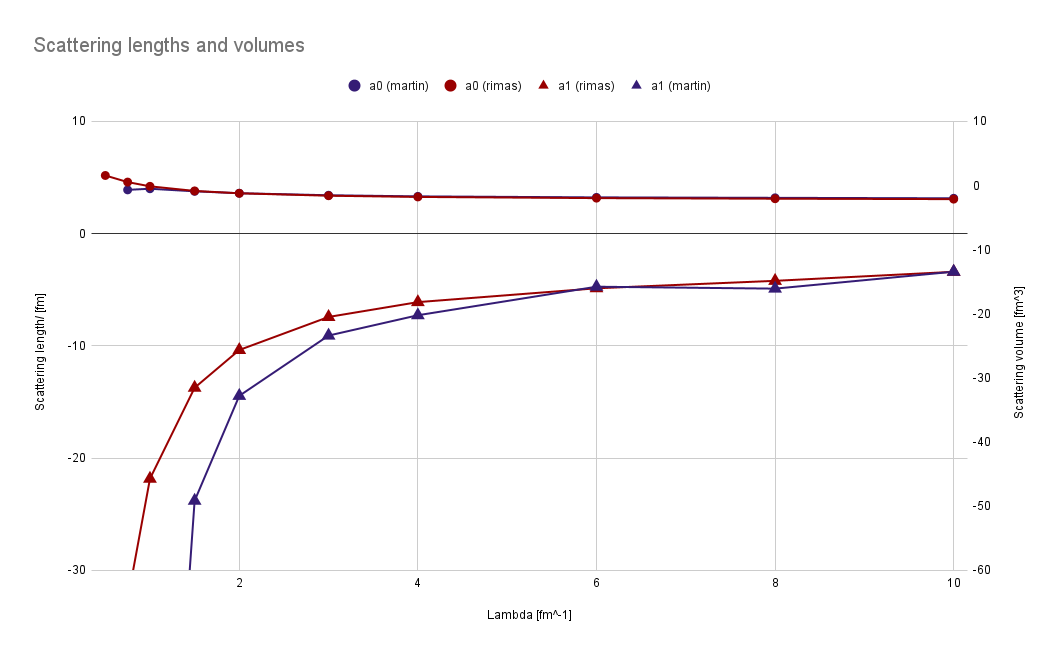
\includegraphics[width=0.95\textwidth]{./Graphs/a0a1} 
\caption{$1^-$ resonant pole in $^4$H}
\label{fig:a0a1}
\end{figure}


Our discussion begins with the analysis of low energy scattering parameters of the $n-^3$H system. 
This system allows for several low-energy states with relative angular momentum $J=1$ between the fragments: $0^-$, $1^-$, and $2^-$; we focus exclusively on the natural parity state: $1^-$. 
We also study the state $0^+$, with relative angular momentum L=$0$. 
This state is Pauli excluded, therefore, we do not expect any resonant or bound state in this channel but we still consider it interesting to study the EFT behavior and as a benchmark among different methods.
In figure \ref{fig:a0a1} we shown the scattering length and volume (relative to $0^+$ and $1^-$ states) calculated using SVM and RIMAS microscopical approaches.
Can be noticed how, for large enough cutoffs, the two methods are compatible.
This was expected since the two calculations use effectively two different regulators due to the presence of an S-wave projected and unprojected two-body potential. 
The difference between the two is more noticeable in the $J^\pi=1^-$ channel as the effect of P-wave interactions is more evident.
The two scattering parameters converge with the cut-off to a finite value. 
This fact is nontrivial since the interparticle interaction converges to a contact potential for large cut-offs.
In fact, $n$ and $^3H$ contain an identical fermion which suppresses any positive parity interaction.
However, the contact nature of the potential allows only particles in relative S-wave to interact. 
The finiteness of $a_0$ and $a_1$ should, therefore, be explained by the mediation of the distinguishable fermions and by the few-body effects.
$a_0$ and $a_1$ converge, empirically, as $1/\lambda$. 
In other words, since the interplay of S-wave interactions can result in a finite interaction in P-wave among few-body clusters, the scattering length/volume remains finite even only including the theory LO.
As a consequence, their cut-off behavior is $\propto1/\Lambda$ as expected by LO observables.
The sign and magnitude of the converged results ($a_0\simeq 3.1$ fm and $a_1\simeq-13(1)$) indicate the absence of boundstates, but the $a_1$ magnitude might indicate the presence of a shallow pole in the $1^-$ system.
It is also interesting to notice that the effective range for $0^+$ and $1^-$ remains also finite ($r_0\simeq2$ fm and $r_1\simeq1$ fm respectively).
This is also expected since, despite the nucleon-nucleon interaction is of contact nature, the size of the fragments remains finite, allowing for an inter-fragment long-range effect.
%

While arguably the best method to extract phaseshifts and resonance positions, the microscopic approach becomes more and more complicated and unfeasible when the number of particles is increased. 
For this, we would like to tackle the same problem from a different perspective: using the RGM formalism.
RGM intrinsically contains an approximation in the form of a simplified few-body wave function of one of the fragments.
It is, however, easily extendable to larger systems.
In our case, RGM transform a four-body problem into a simplified two-fragment one at the price of 




%
%
\begin{figure}
\centering
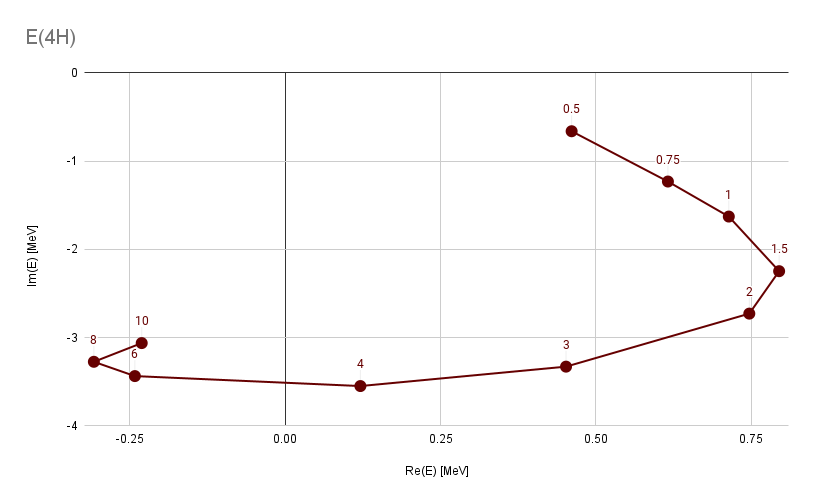
\includegraphics[width=0.95\textwidth]{./Graphs/E4H} 
\caption{$1^-$ resonant pole in $^4$H}
\label{fig:Resonance_pole}
\end{figure}
%

%
The second step in our calculation is the determination of the $J^\pi=1^-$ nuclear resonance position in the Energy complex plane. 
This has been done using the ACCC method starting from "RIMAS" numerical method. 
In figure \ref{fig:Resonance_pole}, the evolution of such pole can be follow to pass the threshold energy $B_{t}=8.484$ MeV ($Re(E)=0$ in the plot) to stabilize around $E_{n-t}=-8.7-i\,3.1$ for cutoffs greater than $6$ fm$^{-1}$.
This represents a shallow and broad subthreshold resonance. 
The presence of such a state and especially its stability (in this case expressed as a pole that does not run to infinite energy increasing the cut-off) is not trivial for the same reasons as one might not expect scattering length/volumes larger than zero.
%
Therefore, this proves that the theory is able to predict shallow states in systems with mixed symmetry. 
However, the position of the LO EFT pole appears to not be compatible with the physical resonance in $^4H$: ??? ($E_{n-t}=8.17+i\,6.73$). %\cite{http://tunlweb.tunl.duke.edu/nucldata/ourpubs/04_1992.pdf}. where does this come from? ???
Nonetheless, the theory is only tested at LO where the relevant operators to describe such states are not been yet introduced.
It is not in principle problematic that the LO pole is not consistent with the experimental data since including the subleading orders (NLO and N$^2$LO) can, even in a perturbative treatment of the expansion, relocate it in the correct position.
However, in this process one should be careful that the insertion of the subleading operators does not shift unreasonably, neither too much nor in the wrong direction, any of the other observables (e.g. the $^4He$ energy or the $n-^2H$ phaseshifts). 
At the current knowledge of the authors, no studies have ever been done in this sense and the possibility of a consistent correction of a resonant pole in therms of powerconting hierarchy remains to be demonstrated.
%




\subsection*{Universality}

%
In the framework of universal systems, in which the two-body scattering length is divergent, the scattering volume of $n-^3H$ follows an identical pattern as before, but with a convergent value of $\sim4$ fm$^3$.
This can be compared to the typical coordinate scale of the system, which, in this case, is uniquely identifiable with the three-body scale $R_3=(-2mE_3/\hbar^2)^{-1/2}\simeq 6$ fm. 
We find that $(a_1)^{-1/3}/R_3 \simeq  1/4$, which is a small, but still natural ratio.

** here I have some discrepancies (martin A11 is twice Rimas A11)
\begin{figure}
\centering
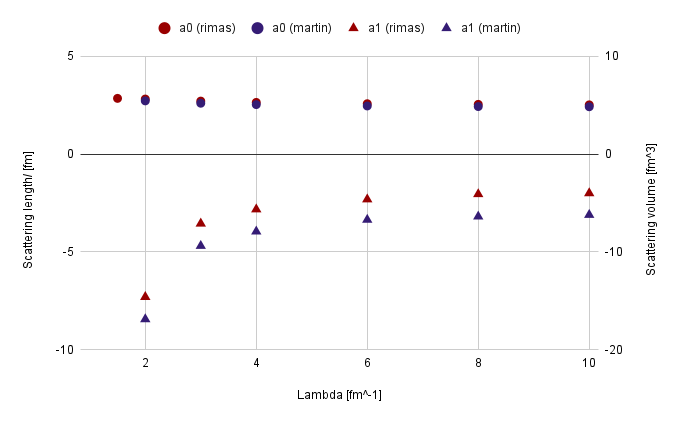
\includegraphics[width=0.95\textwidth]{./Graphs/unitarityA} 
\caption{Temporary: unitary scattering lengths / volume}
\label{fig:Resonance_pole}
\end{figure}
**[martin pole and data for unitarity]**






\section{conclusion}




\bibliographystyle{ieeetr}
%elsarticle-harv}
\bibliography{bibi.bib}

\section{Appendix: Resonating group method and interactions}
\end{document}